%*----------- SLIDE -------------------------------------------------------------
\begin{frame}[t]{Metodologia - Avaliação do modelo}
    Para analisar o modelo criado, os autores adotadaram ao todo quatro métricas 
    \vspace{0.4cm}

    O parâmetro \textbf{\textit{"Accuracy"}}  representa a fração das predições feitas corretamente
    \vspace{0.4cm}

    A \textbf{\textit{"Precision"}} é a razão entre as predições positivas corretas dentre todas as predições positivos 
    \begin{table}[]
        \vspace{0.8cm}
        \centering
        \begin{tabular}{ll}
            \begin{math} Accuracy = \frac{Number\,of\,correct\,predictions}{Total\,number\,of\,predictions} \end{math} 
            &
            \begin{math} Precision = \frac{True\,Positive}{True\,Positive + False\,Positive} \end{math} 
        \end{tabular}
    \end{table}
    
%*----------- notes
    \note[item]{Notes can help you to remember important information. Turn on the notes option.}
\end{frame}

%*----------- SLIDE -------------------------------------------------------------
\begin{frame}[t]{Metodologia - Avaliação do modelo}
    O parâmetro \textbf{\textit{"Recall"}} é a habilidade do modelo de encontrar os positivos verdadeiros
    \vspace{0.4cm}
    
    A \pmb{"\begin{math} F_1Score \end{math}"} é a média harmônica pondera entre os parâmetros \textit{"Precision"} e \textit{"Recall"}
    \begin{table}[]
        \vspace{0.8cm}
        \centering
        \begin{tabular}{ll}
            \begin{math} Recall = \frac{True\,Positive}{True\,Positive + False\,Negative} \end{math}
            &
            \begin{math} F_1Score = 2\cdot\frac{Precision \cdot Recall}{Precision + Recall} \end{math}
        \end{tabular}
    \end{table}
    
%*----------- notes
    \note[item]{Notes can help you to remember important information. Turn on the notes option.}
\end{frame}

%*----------- SLIDE -------------------------------------------------------------
\begin{frame}[t]{Metodologia - As amostras}
    Para treino do modelo foram consideradas as 3 seguintes abaixo
    \begin{columns}[t]
        \column{.35\linewidth}
        \begin{center}
            %\centerline{
                \begin{figure}
                    %\roundpic[xshift=0cm,yshift=0cm]{5cm}{8cm}{dying-blueberry.jpg}
                    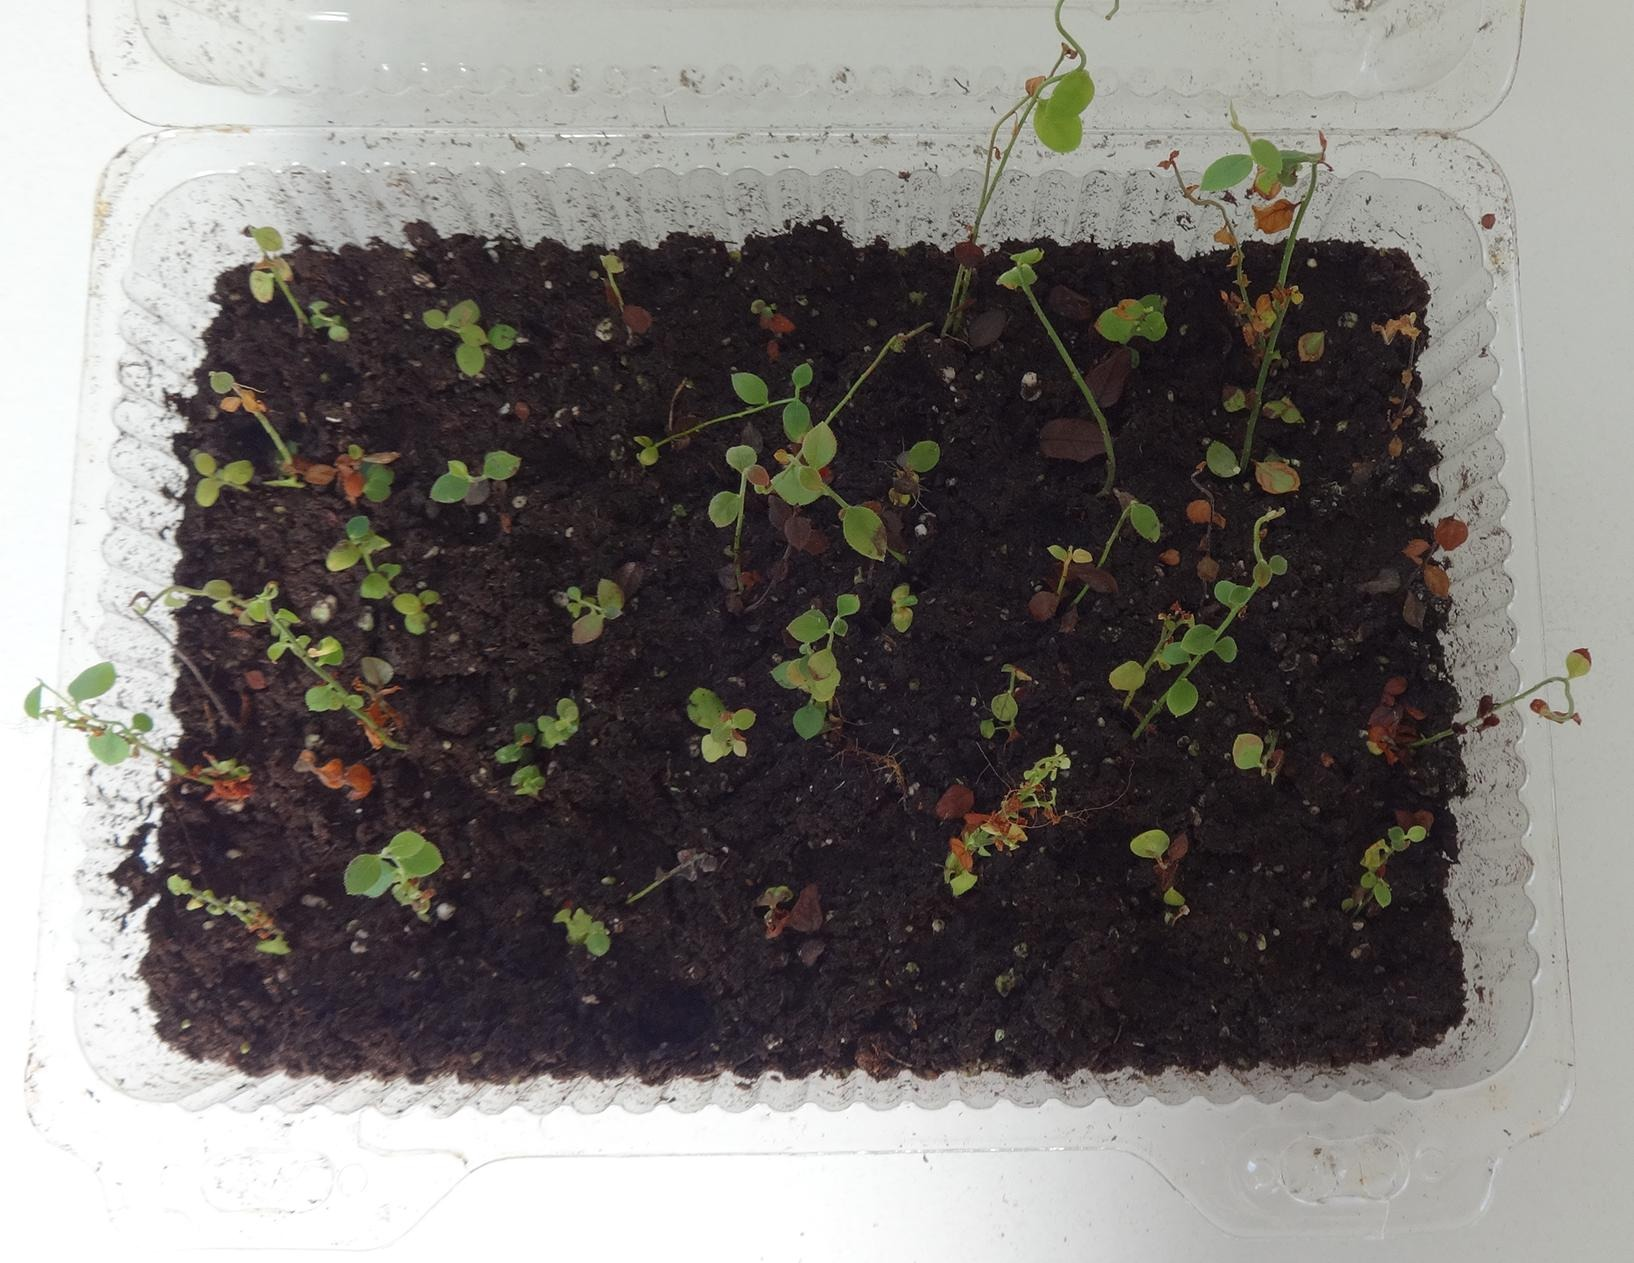
\includegraphics[width=0.85\textwidth]{bandeja-com-plantas.jpg}
                    \caption{Bandeja com plantas}
                \end{figure}
            %}
        \end{center}

        \column{.35\linewidth}
        \begin{center}
            %\centerline{
                \begin{figure}
                    %\roundpic[xshift=0cm,yshift=0cm]{5cm}{8cm}{dying-blueberry.jpg}
                    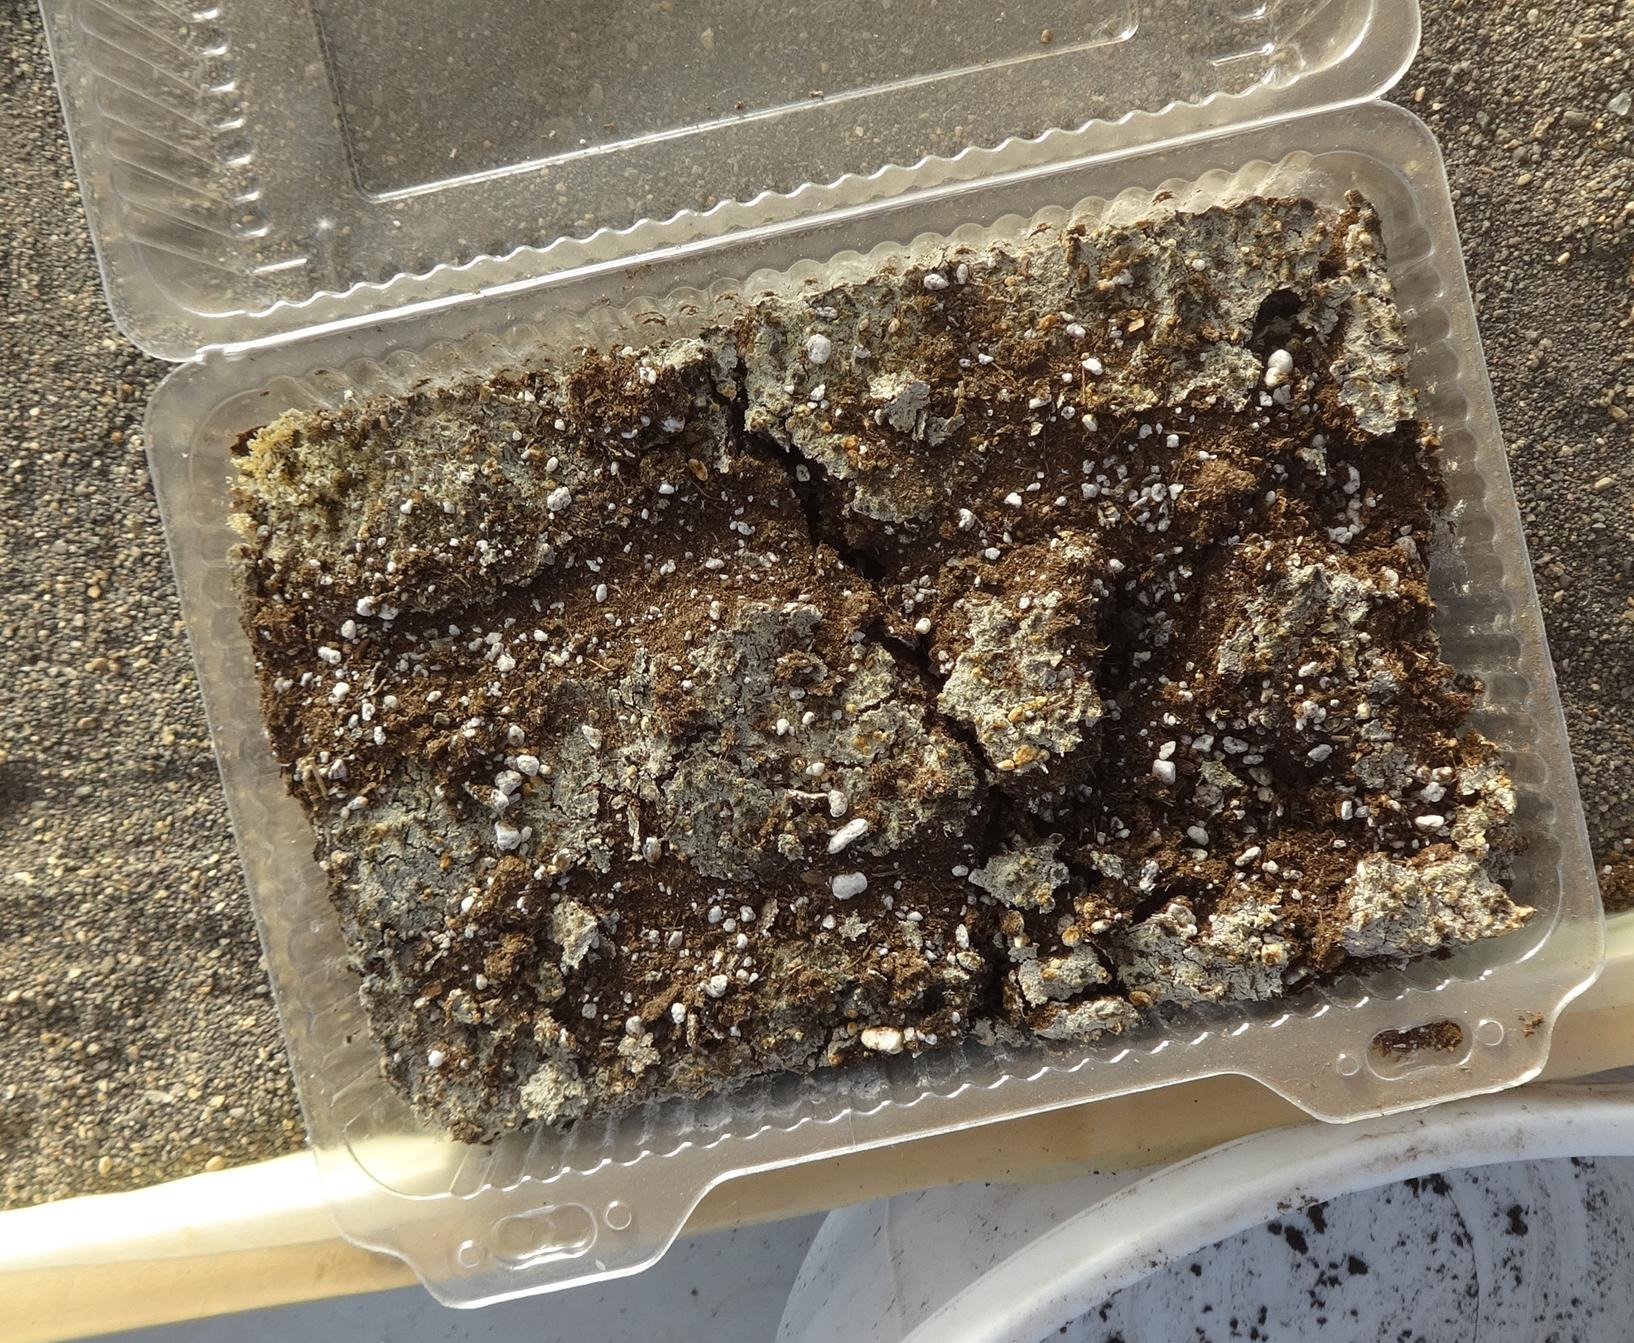
\includegraphics[width=0.8\textwidth]{bandeja-vazia.jpg}
                    \caption{Bandeja sem plantas}
                \end{figure}
            %}
        \end{center}

        \column{.35\linewidth}
        \begin{center}
            %\centerline{
                \begin{figure}
                    %\roundpic[xshift=0cm,yshift=0cm]{5cm}{8cm}{dying-blueberry.jpg}
                    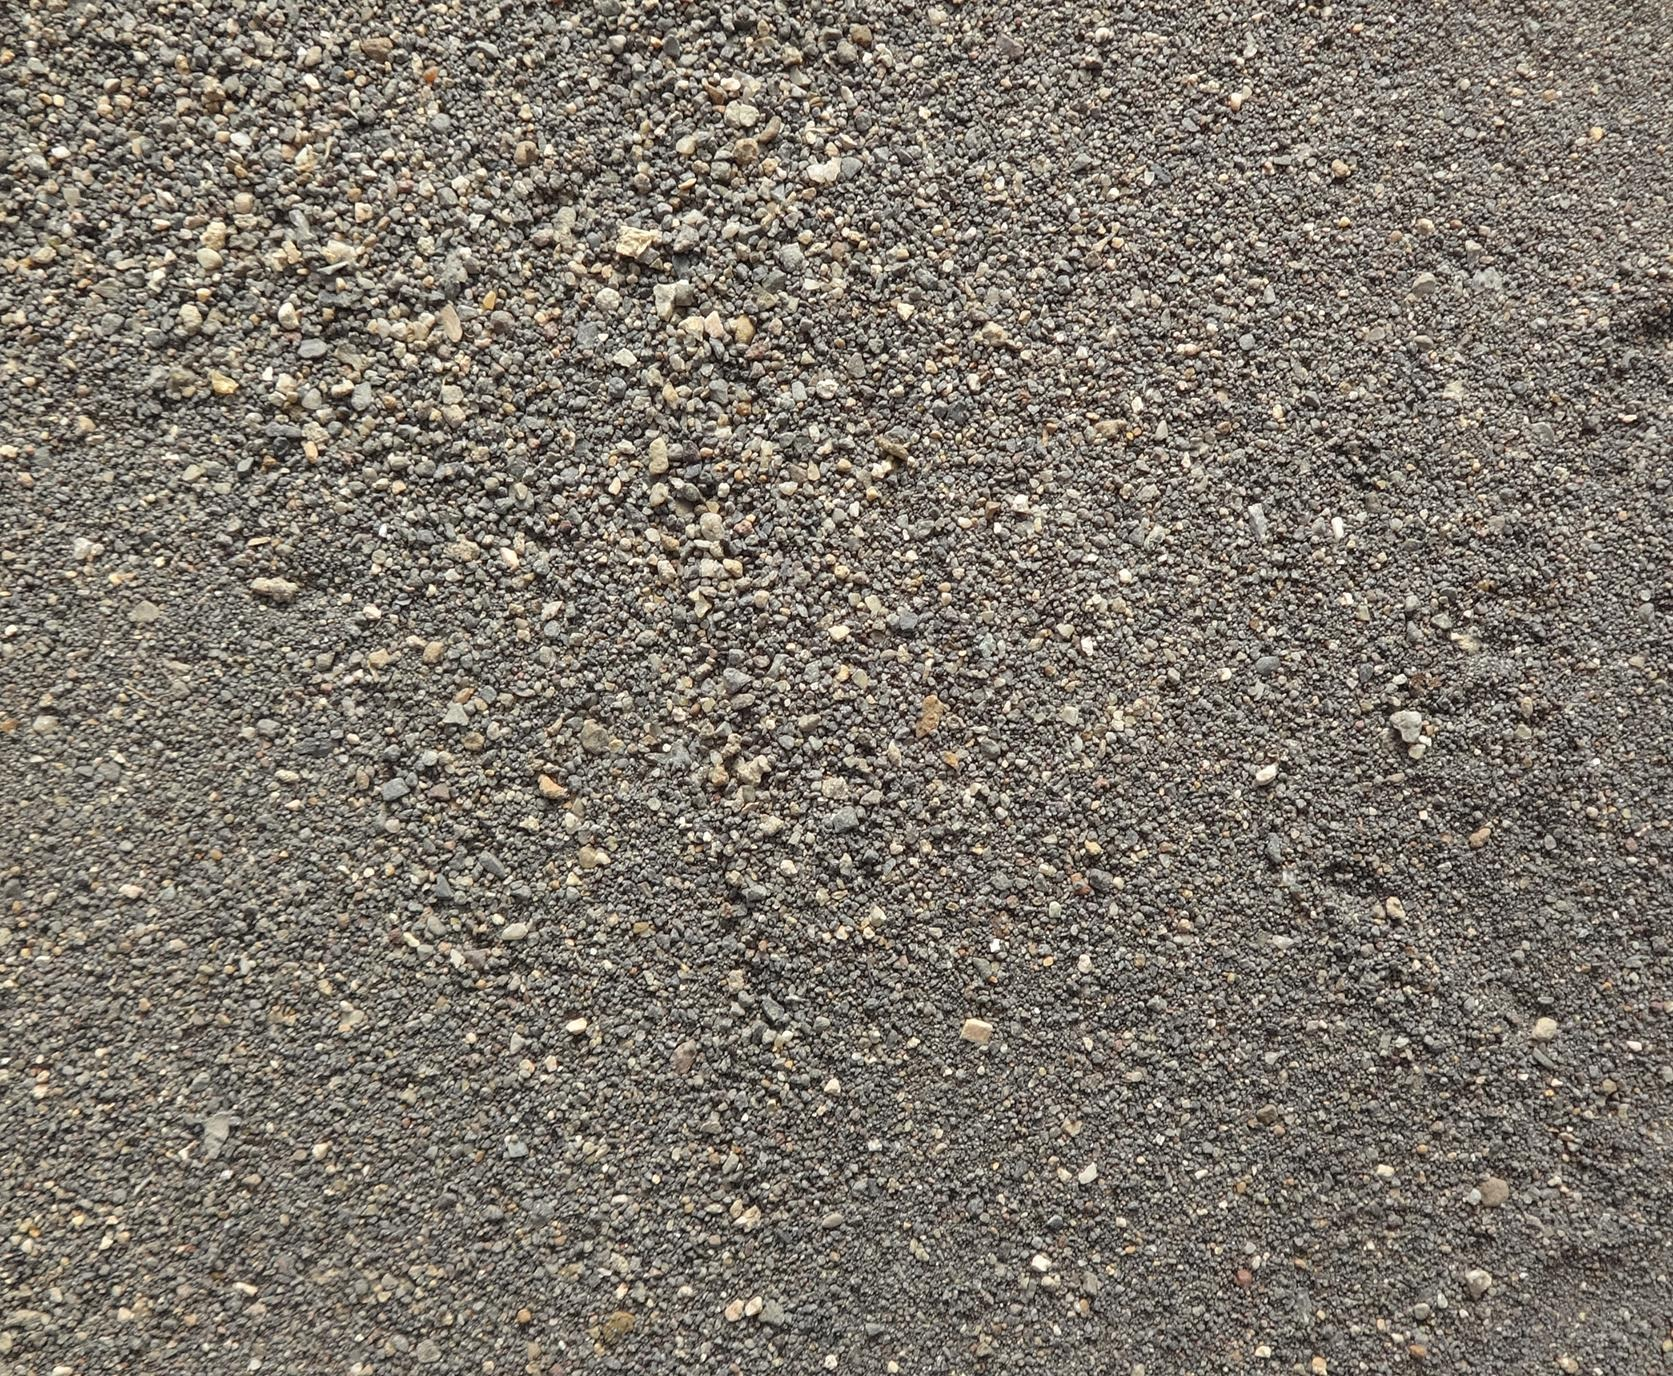
\includegraphics[width=0.8\textwidth]{bandeja-sem.jpg}
                    \caption{Espaço sem bandejas}
                \end{figure}
            %}
        \end{center}
    \end{columns}
%*----------- notes
    \note[item]{Notes can help you to remember important information. Turn on the notes option.}
\end{frame}


%*----------- SLIDE -------------------------------------------------------------
\begin{frame}[t]{Metodologia - As amostras}
    Distribuição das imagens usadas no experimento (valores totais em negrito)
    \begin{table}[]
        \centering
        \begin{tabular}{cccc}
        \hline
        \multirow{2}{*}{\vspace{-1cm}\textit{Estágios}}                                                    & \multicolumn{3}{c}{\textit{Classes}}                                                                                                                                                                              \\ \cline{2-4} 
                                                                                            & \textit{\begin{tabular}[c]{@{}c@{}}Bandejas com\\ Legacy blueberry\\ vivas\end{tabular}} & \textit{\begin{tabular}[c]{@{}c@{}}Bandeja sem \\ Legacy blueberry \\ vivas\end{tabular}} & \textit{Sem bandeja} \\ \hline
        \textit{Treinamento}                                                                   & 56                                                                                            & 56                                                                                             & 56               \\
        \textit{Validação}                                                                 & 18                                                                                            & 18                                                                                             & 18               \\
        \textit{Predição}                                                                 & 12                                                                                            & 12                                                                                             & 12               \\
        \textbf{\begin{tabular}[c]{@{}c@{}}Número total de\\ imagens por classe\end{tabular}} & \textbf{86}                                                                                            & \textbf{86}                                                                                             & \textbf{86}               \\
        \textbf{\begin{tabular}[c]{@{}c@{}}Número total de\\ imagens\end{tabular}}           & \multicolumn{3}{c}{\textbf{258}}                                                                                                                                                                                  \\ \hline
        \end{tabular}
    \end{table}
%*----------- notes
    \note[item]{Notes can help you to remember important information. Turn on the notes option.}
\end{frame}

% FALTA: contexto(onde e como), mapa, solução